\documentclass[11pt,a4paper]{article}
\usepackage[left=2.5cm,right=2cm, bottom=2cm]{geometry}
\usepackage[utf8]{inputenc}
\usepackage{amsmath}
\usepackage{amsfonts}
\usepackage{amssymb}
\usepackage{amsfonts}
\usepackage{amsmath}
\usepackage{graphicx}
\usepackage{subfigure}
\usepackage{color}
\usepackage{abstract}
\usepackage{float}
\usepackage[toc,page]{appendix}
\usepackage{hyperref}
\usepackage{fancyhdr}
\usepackage{algorithm} 
\usepackage{algpseudocode} 
\usepackage{listings}
\usepackage{xcolor} % for setting colors
% set the default code style
\lstset{
	frame=tb, % draw a frame at the top and bottom of the code block
	tabsize=4, % tab space width
	showstringspaces=false, % don't mark spaces in strings
	numbers=left, % display line numbers on the left
	commentstyle=\color{green}, % comment color
	keywordstyle=\color{blue}, % keyword color
	stringstyle=\color{red} % string color
}

\pagestyle{fancy}
\fancyhf{}
\rhead{\today}
\lhead{\bfseries Alexander Leitner 01525882}
\rfoot{}



\begin{document}
\begin{center}
	\fontsize{24pt}{10pt}\selectfont
	\textsc{\textbf{Computational Science on Many-Core Architectures  Exercise 7}}
\end{center}
\section*{Example 1 Dot Product with OpenCL (4 Points)}
\subsection*{a)}
\begin{lstlisting}[language=C++, caption={opencl kernel}]
const char *my_opencl_program = ""
"__kernel void vec_mult(__global double *x,\n"
"                      __global double *y,\n"
"                      __global double *result,\n"
"                      unsigned int N\n)"
"{\n"
"  for (unsigned int i  = get_global_id(0);\n"
"                    i  < N;\n"
"                    i += get_global_size(0))\n"
"    result[i] = x[i] * y[i];\n"
"}"; 
\end{lstlisting}
\noindent
This opencl kernel only multiplies the single entries and stored the results in the result vector.
\begin{lstlisting}[language=C++, caption={Benchmark for the opencl}]
for (int i = 0;i < anz; i++)
{
	//
	// Set kernel arguments:
	//
	timer.reset();
	err = clSetKernelArg(my_kernel, 0, sizeof(cl_mem),  
	(void*)&ocl_x); OPENCL_ERR_CHECK(err);
	
	err = clSetKernelArg(my_kernel, 1, sizeof(cl_mem),  
	(void*)&ocl_y); OPENCL_ERR_CHECK(err);
	
	err = clSetKernelArg(my_kernel, 2, sizeof(cl_mem),  
	(void*)&ocl_result); OPENCL_ERR_CHECK(err);
	
	err = clSetKernelArg(my_kernel, 3, sizeof(cl_uint), 
	(void*)&vector_size); OPENCL_ERR_CHECK(err);
	
	//
	// Enqueue kernel in command queue:
	//
	err = clEnqueueNDRangeKernel(my_queue, my_kernel, 1, 
	NULL, &global_size, &local_size, 0, NULL, NULL); OPENCL_ERR_CHECK(err);
	
	// wait for all operations in queue to finish:
	err = clFinish(my_queue); OPENCL_ERR_CHECK(err);
}
opencl_time = timer.get();
std::cout << "Time for opencl kernel: " << opencl_time/anz << std::endl;
\end{lstlisting}
The for loop is only for the benchmark and $anz = 100$.
I only add the line 13 and 14 to set the buffer for the result vector.
\begin{lstlisting}[language=C++, caption={CUDA kernel}]
__global__ void GPU_dot (double *x, double *y, double *dot, unsigned int N)
{
	unsigned int ind = threadIdx.x + blockDim.x*blockIdx.x;
	unsigned int str = blockDim.x*gridDim.x;
	
	double tmpsum = 0.0;
	while(ind < N)
	{
		tmpsum = x[ind]*y[ind];
		ind += str;
	}
	dot[threadIdx.x] = tmpsum;
}
\end{lstlisting}

\begin{lstlisting}[language=C++, caption={CUDA benchmark}]
timer.reset();
for (int i = 0;i < anz; i++)
{
	GPU_dot<<<128, 128>>>(cuda_X, cuda_Y, cuda_dot_GPU, N);
	cudaDeviceSynchronize();
	cudaMemcpy(dot_GPU, cuda_dot_GPU, sizeof(double), cudaMemcpyDeviceToHost);
}
//cudaMemcpy(dot_GPU, cuda_dot_GPU, sizeof(double), cudaMemcpyDeviceToHost);
GPU_time = timer.get();
std::cout << "Time for GPU kernel: " << GPU_time/anz << std::endl;
\end{lstlisting}
\newpage
\begin{lstlisting}[language=C++, caption={CPU kernel}]
void CPU_dot(ScalarType *x, ScalarType *y, ScalarType *result,
     unsigned int N)
{
	for (int i = 0; i < N; i++)
	{
		result[i] = x[i] * y[i];
	}
}
\end{lstlisting}

\begin{lstlisting}[language=C++, caption={CPU benchmark}]
timer.reset();
for (int i = 0;i < anz; i++)
{
	CPU_dot(X, Y, dot_CPU, N);
}
CPU_time = timer.get();
std::cout << "Time for CPU kernel: " << CPU_time/anz << std::endl;
\end{lstlisting}
\begin{center}
\begin{minipage}[t]{0.49\textwidth}
	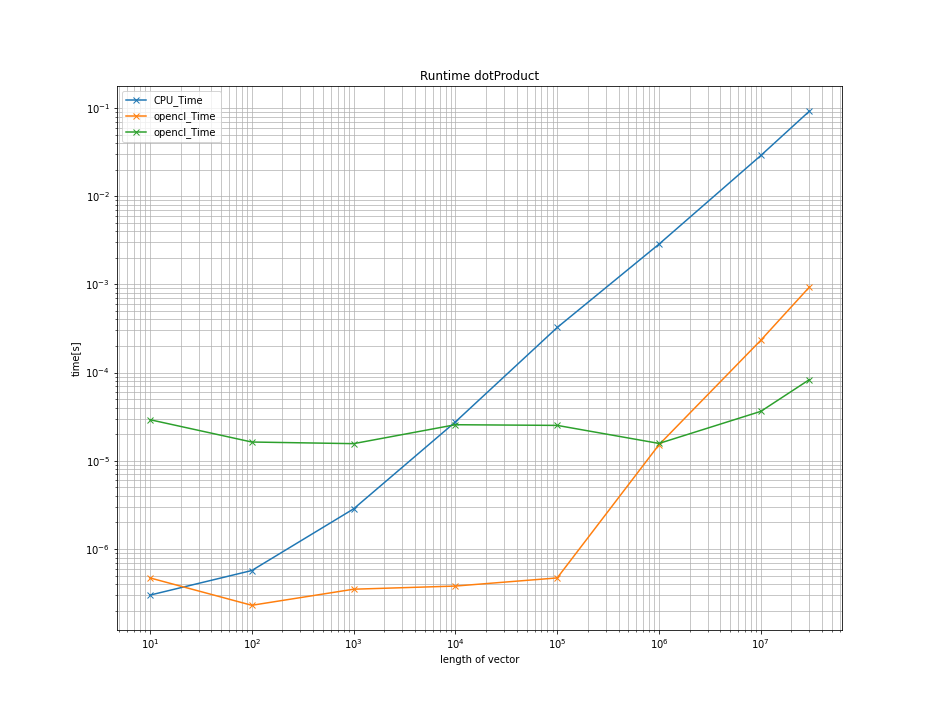
\includegraphics[width=\textwidth]{Bilder/Runtime_dotProduct}
\end{minipage}
\begin{minipage}[t]{0.49\textwidth}
	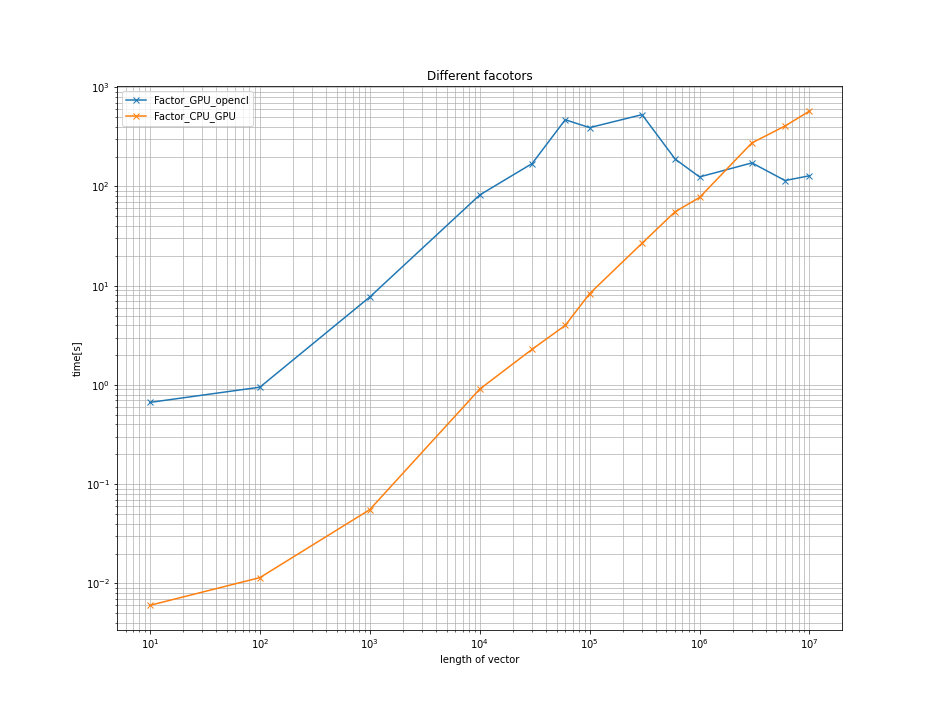
\includegraphics[width=\textwidth]{Bilder/diff_factor}
\end{minipage}	
\end{center}

\noindent
On the left we could see that the different runtimes for the same number of entries of a vector and apply the dot-product on it. For the GPU-times it is not clear why the times are like this. I also switch the mode of the machine to the GTX 1080. On the right side I plotted the different factros which one is faster opencl or CPU and GPU or CPU. At a certain point opencl is over 200 times faster than the CPU one.

\begin{center}
	\begin{minipage}[t]{0.49\textwidth}
		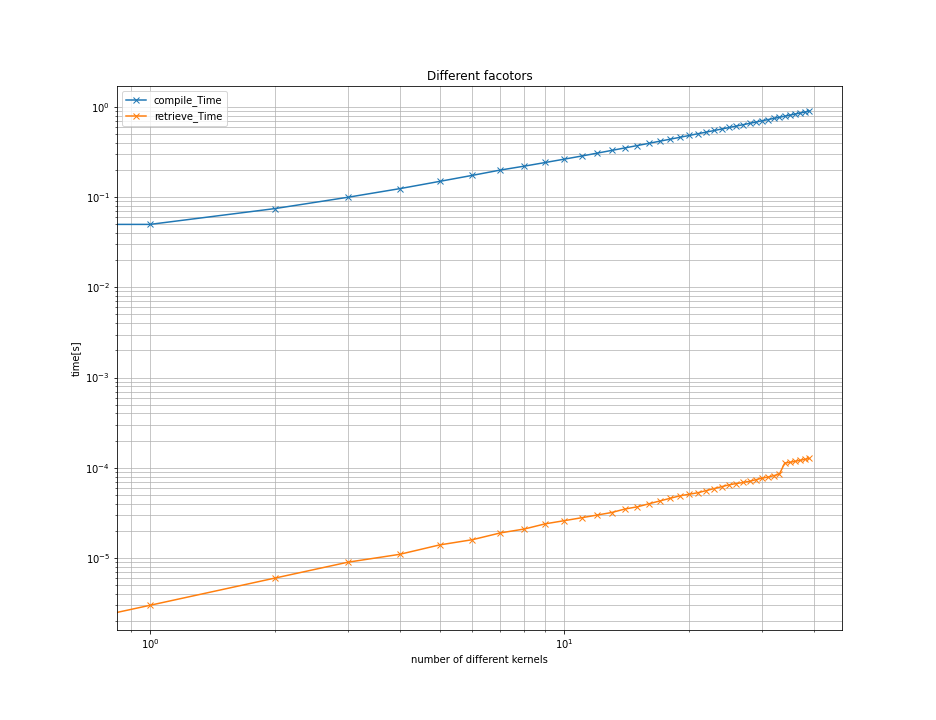
\includegraphics[width=\textwidth]{Bilder/Time_to_compile_and_clean}
	\end{minipage}
\end{center}

\noindent
The time to create the kernels is linear with the numbers of $M$ different kernels and also the time to retrive it. The second case is much faster than the fist.\\
For 1.4 I tried first to write a routine which adds a line with respect to a given number of $M$ to creat every time a different kernel and to measure the time. I tried this with a string implementation. That does not work prooaly because the decleration at the begin of the provided code is a $const\,\,\,char$ and I got errors that I could not change a $const\,\,\,char$ for that. Then I tried to implement it with $char$ datatyps and that also does not work. So I wrote 100 different kernels with if conditions and add a line "d = 0;" which does not affect the implementation from the dot product and so I measures the time. My code is 4500 lines long so dont affraid I could not find a better solution.
	
\end{document}